\chapter{phase transitions: criticality, universality, and scaling}
\begin{itemize}
	\item 热力学系统可以分为两类: noninteracting \& interacting.
	
	\item noninteracting 的系统包括: the specific heat of gases (section \ref{1.2} and \ref{6.4}); the specific heat of solids (section \ref{7.4}); chemical equilibrium in an ideal gas or a dilute solution (section \ref{6.5}); condensation of an ideal Bose gas (section \ref{7.1} and \ref{7.2}); spectral distribution of the blackbody radiation (section \ref{7.3}); the free electron theory of metals (section \ref{8.3}); the phenomenon of paramagnetism (section \ref{3.7} and \ref{8.2}).
	\begin{itemize}
		\item 除了 Bose--Einstein condensation 之外, 所有这些系统的 thermodynamic functions 都是光滑的.
	\end{itemize}
	
	\item interacting 的系统包括: the condensation of gases; the melting of solids; the coexistence of phases (especially near a critical point); mixtures and solutions (包括 the onset of phase separation); ferromagnetism and antiferromagnetism; the order--disorder transitions in alloys; the superfluid transition from liquid He I to liquid He II; transition from a normal to a superconducting material.
	\begin{itemize}
		\item interacting 的系统, 经常会遇到 thermodynamic functions 具有 analytic discontinuities or singularities 的情况, 相应地, 会遇到各种 phase transitions.
	\end{itemize}
\end{itemize}

\section{general remarks on the problem of condensation}
\begin{itemize}
	\item 对任何热力学系统, 都有
	\begin{equation}
		\Big( \frac{\partial P'}{\partial v} \Big)_{V, T} = - \frac{k_B T}{v^2} \frac{\braket{N}}{\braket{(\Delta N)^2}} \leq 0,
	\end{equation}
	其中 $P'$ 定义为
	\begin{equation}
		P' := \frac{k_B T}{V} \ln Z_\text{GC} \equiv - \frac{\Phi_\text{G}}{V},
	\end{equation}
	对于 homogeneous system (注意 multiphase systems 也可以是 homogeneous, 但要忽略表面效应) 有 $P' = P$.
	
	\begin{tcolorbox}[title=calculation:]
		注意到
		\begin{equation}
			- \frac{V}{N^2} \Big( \frac{\partial P'}{\partial v} \Big)_{T, V} = \Big( \frac{\partial P'}{\partial N} \Big)_{T, V} = - \frac{1}{V} \Big( \frac{\partial \Phi_\text{G}}{\partial N} \Big)_{T, V},
		\end{equation}
		且
		\begin{equation}
			\Big( \frac{\partial \Phi_\text{G}}{\partial N} \Big)_{T, V} = - N \Big( \frac{\partial \mu}{\partial N} \Big)_{T, V} = - \frac{N}{\big( \frac{\partial N}{\partial \mu} \big)_{T, V}} = - \frac{N}{\beta \braket{(\Delta N)^2}},
		\end{equation}
		最后一个等号用到了 \eqref{4.4.1}.
	\end{tcolorbox}
	
	\item 注意到, 在某些区间 $\braket{(\Delta N)^2} \sim O(N^2)$, 此时
	\begin{equation}
		\Big( \frac{\partial P'}{\partial v} \Big)_{V, T} \sim O(N^{- 1}) \simeq 0.
	\end{equation}
\end{itemize}

\section{condensation of a van der Waals gas}
\subsection{mean field estimate}
\begin{itemize}
	\item 考虑气体分子之间具有相互作用, 那么系统的 partition function 为
	\begin{align}
		Z_\text{C}(T, V, N) &= \frac{1}{N!} \int \frac{d^{3 N} p d^{3 N} q}{h^{3 N}} e^{- \beta \sum_{i = 1}^N \frac{p_i^2}{2 m}} e^{- \beta \sum_{i > j} u(q_i - q_j)} \notag \\
		&\simeq \frac{1}{N! \lambda^{3 N}} \Big( V - \frac{N \Omega}{2} \Big)^N e^{\beta \frac{V}{2 v^2} u}.
	\end{align}
	
	\begin{tcolorbox}[title=calculation:]
		考虑
		\begin{equation}
			\sum_{i > j} u(\vec{q}_i - \vec{q}_j) = \frac{1}{2} \int d^3 r_1 d^3 r_2 \, n(\vec{r}_1) n(\vec{r}_2) u(\vec{r}_1 - \vec{r}_2),
		\end{equation}
		其中
		\begin{equation}
			n(\vec{r}) = \sum_{i = 1}^N \delta^{(3)}(\vec{r} - \vec{q}_i) \Longrightarrow \int d^3 r \, n(\vec{r}) = N,
		\end{equation}
		作 approximation of uniform density, 那么
		\begin{equation}
			n(\vec{r}) \simeq \frac{N}{V} \Longrightarrow \sum_{i > j} u(\vec{q}_i - \vec{q}_j) \simeq \frac{V}{2 v^2} \int d^3 r \, u(\vec{r}),
		\end{equation}
		注意到
		\begin{equation}
			u(\vec{r}) = u(r) = \begin{dcases}
				\infty & r < \sigma \\
				< 0 & r > \sigma
			\end{dcases} \quad \text{and} \quad \int_\sigma^\infty u(r) 4 \pi r^2 dr = - u < 0,
		\end{equation}
		代入
		\begin{equation}
			\sum_{i > j} u(\vec{q}_i - \vec{q}_j) \simeq - \frac{V}{2 v^2} u,
		\end{equation}
		最后, 注意到 (其中 $\Omega = \frac{4 \pi}{3} (2 \sigma)^3$)
		\begin{equation}
			\int d^{3 N} q \simeq V (V - \Omega) \cdots (V - (N - 1) \Omega) \simeq V^N - \frac{N^2}{2} \Omega V^{N - 1} \simeq \Big( V - \frac{N \Omega}{2} \Big)^N,
		\end{equation}
		所以...
	\end{tcolorbox}
	
	\item 得到
	\begin{equation}
		\begin{dcases}
			F = - k_B T \ln Z_\text{C} = N k_B T \Big( - 1 + \ln \frac{n \lambda^3}{1 - \frac{n \Omega}{2}} \Big) - \frac{N^2}{2 V} u \\
			P = - \Big( \frac{\partial F}{\partial V} \Big)_{T, N} = k_B T \Big( \frac{\partial \ln Z_\text{C}}{\partial V} \Big)_{T, N} = \frac{k_B T}{v - \frac{\Omega}{2}} - \frac{u}{2 v^2} \\
			S = N k_B \Big( \frac{5}{2} - \ln \frac{n \lambda^3}{1 - \frac{n \Omega}{2}} \Big) \\
			U = \frac{3}{2} N k_B T - \frac{N^2}{2 V} u \\
			\mu = k_B T \Big( \frac{\frac{n \Omega}{2}}{1 - \frac{n \Omega}{2}} + \ln \frac{n \lambda^3}{1 - \frac{n \Omega}{2}} \Big) - \frac{N}{V} u
		\end{dcases},
	\end{equation}
	且有
	\begin{equation}
		\frac{\Omega}{2} := b, \quad \frac{u}{2} := a.
	\end{equation}
\end{itemize}

\subsection{the van der Waals equation}
\begin{itemize}
	\item van der Waals gas 满足 equation of state 为
	\begin{equation}
		P = \frac{k_B T}{v - b} - \frac{a}{v^2} \quad \text{or} \quad P_r = \frac{8 T_r}{3 v_r - 1} - \frac{3}{v_r^2},
	\end{equation}
	其中 $P_r = \frac{P}{P_c}, v_r = \frac{v}{v_c}, T_r = \frac{T}{T_c}$, 且
	\begin{equation}
		P_c = \frac{a}{27 b^2}, \quad v_c = 3 b, \quad k_B T_c = \frac{8 a}{27 b}.
	\end{equation}
	
	\item 注意到 $\mu_\text{liquid} = \mu_\text{gas}$, 因此
	\begin{equation}
		\frac{8}{9} T_r \Big( \frac{1}{3 v_{r, \text{liquid}} - 1} - \frac{1}{3 v_{r, \text{gas}} - 1} + \ln \frac{3 v_{r, \text{gas}} - 1}{3 v_{r, \text{liquid}} - 1} \Big) - \Big( \frac{1}{v_{r, \text{liquid}}} - \frac{1}{v_{r, \text{gas}}} \Big) = 0,
	\end{equation}
	有
	\begin{equation} \label{10.2.13}
		v_{r, \text{liquid}} = \frac{1 + f(y) e^y}{3 f(y) e^y}, \quad v_{r, \text{gas}} = \frac{1 + f(y) e^{- y}}{3 f(y) e^{- y}}, \quad f(y) = \frac{y \cosh y - \sinh y}{\cosh y \sinh y - y},
	\end{equation}
	并且 $T_r(y = 0) = 1, f(y = 0) = \frac{1}{2}$.
	\begin{itemize}
		\item 具体的计算细节可以参考 Wikipedia page: \href{https://en.wikipedia.org/wiki/Van_der_Waals_equation#Saturation}{van der Waals equation: saturation}.
		
		\item $T_r(y), v_{r, \text{liquid}}(y), v_{r, \text{gas}}(y), P_r(y), f(y)$ 的函数图像如下图:
		
		\begin{figure}[H]
			\centering
			\includegraphics[scale=0.8]{figures/plot of T_r(y), v_{r, text{liquid}}(y), v_{r, text{gas}}(y), P_r(y), and f(y).pdf}
			\caption{plot of $T_r(y), v_{r, \text{liquid}}(y), v_{r, \text{gas}}(y), P_r(y)$, and $f(y)$.}
		\end{figure}
	\end{itemize}
	
	\item van der Waals gas 的 isotherms 如下图所示:
	
	\begin{figure}[H]
		\centering
		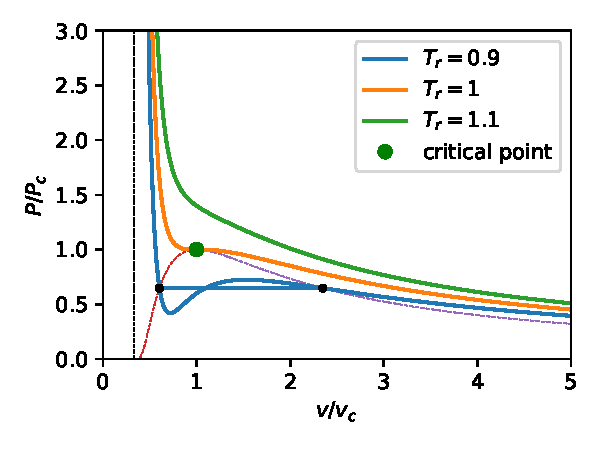
\includegraphics[scale=0.8]{figures/isotherms of the van der Waals gas.pdf}
		\caption{isotherms of the van der Waals gas.}
	\end{figure}
\end{itemize}

\subsection{critical exponents and fluctuations}
\begin{itemize}
	\item 根据 \eqref{10.2.13}, 在 critical point 附近, $T_r < 1$ 时, 有
	\begin{equation}
		v_{r, \text{liquid}} \simeq 1 - \frac{\Delta}{2}, \quad v_{r, \text{gas}} \simeq 1 + \frac{\Delta}{2},
	\end{equation}
	得到
	\begin{equation}
		T_r \simeq 1 - \frac{1}{16} (v_{r, \text{gas}} - v_{r, \text{liquid}})^2 \iff v_\text{gas} - v_\text{liquid} \sim (T_c - T)^\beta, \beta = \frac{1}{2}.
	\end{equation}
	
	\item 因为在 critical point $\big( \frac{\partial P}{\partial v} \big)_{T, N} = \big( \frac{\partial^2 P}{\partial v^2} \big)_{T, N} = 0$, 所以
	\begin{equation}
		P - P_c \sim (v - v_c)^\delta, \delta = 3 \Longrightarrow \kappa_T = - \frac{1}{v} \Big( \frac{\partial v}{\partial P} \Big)_{T, N} \sim (T - T_c)^{- \gamma}, \gamma = 1,
	\end{equation}
	可见, 在 critical point $\kappa_T \rightarrow \infty$, 根据 \eqref{4.4.2}, 直接后果就是
	\begin{equation}
		\braket{(\Delta N)^2} \rightarrow \infty.
	\end{equation}
\end{itemize}

\section{the Ising model}
\begin{itemize}
	\item 考虑一个 $D$ 维 lattice, 含有 $N$ 个 sites, 每个 lattice site 可以处于两个状态 $s_i = \pm 1$.
	
	\item 系统的能量为
	\begin{equation}
		E\{s_i\} = - B \sum_i s_i - J \sum_{\braket{i j}} s_i s_j,
	\end{equation}
	其中 $\braket{i j}$ 表示 nearest neighbor pairs.
	\begin{itemize}
		\item $J > 0$, 系统称为 ferromagnet (我们只考虑这种情况); $J < 0$, 系统称为 anti-ferromagnet.
		
		\item 用 $q$ 表示每个 lattice site 拥有的 nearest neighbors 数量, 称为 coordination number.
		
		\item $D = 1$, 那么 $q = 2$; $D = 2$ 的 square lattice, 那么 $q = 4$; $D = 2$ 的 triangular lattice, 那么 $q = 6$.
	\end{itemize}
	
	\item 系统的 partition function 为
	\begin{equation}
		Z_\text{C}(T, B, N) = \sum_{\{s_i\}} e^{- \beta E\{s_i\}}.
	\end{equation}
	
	\item 那么, 系统的 magnetization 为
	\begin{equation}
		\braket{m} \equiv \frac{1}{N} \braket{\sum_i s_i} = \frac{1}{N \beta} \frac{\partial}{\partial B} \ln Z_\text{C}(T, B, N) \equiv - \frac{1}{N} \Big( \frac{\partial F}{\partial B} \Big)_{T, N},
	\end{equation}
	并且 $m \in [- 1, 1]$.
	
	\item 分别用 $N_{\uparrow, \downarrow}$ 表示处于 $\uparrow, \downarrow$ 态的 lattice sites 数量, 以及 $N_{\braket{\uparrow \uparrow}, \braket{\uparrow \downarrow}, \braket{\downarrow \downarrow}}$ 表示三种 nearest neighbors 的数量, 那么 (可以选取 $N_\uparrow, N_{\braket{\uparrow \uparrow}}$ 为独立变量)
	\begin{equation}
		\begin{dcases}
			N_\uparrow + N_\downarrow = N \\
			q N_\uparrow = 2 N_{\braket{\uparrow \uparrow}} + N_{\braket{\uparrow \downarrow}} \\
			q N_\downarrow = 2 N_{\braket{\downarrow \downarrow}} + N_{\braket{\uparrow \downarrow}}
		\end{dcases} \Longrightarrow N_{\braket{\cdot \cdot}} = \frac{q}{2} N,
	\end{equation}
	以及
	\begin{equation}
		\begin{dcases}
			E(N_\uparrow, N_{\braket{\uparrow \uparrow}}) = - B (2 N_\uparrow - N) - J \Big( \frac{q}{2} N - 2 q N_\uparrow + 4 N_{\braket{\uparrow \uparrow}} \Big) \\
			m = 2 \frac{N_\uparrow}{N} - 1
		\end{dcases}.
	\end{equation}
\end{itemize}

\subsection{mean field theory}
\begin{itemize}
	\item 假设 lattice site 处于 spin-up 和 spin-down 的概率与其 nearest neighbor 的状态无关, 那么
	\begin{equation}
		N_{\braket{\uparrow \downarrow}} \approx N_{\braket{\cdot \cdot}} \Big( \frac{N_\uparrow}{N} \frac{N_\downarrow}{N} + \frac{N_\downarrow}{N} \frac{N_\uparrow}{N} \Big) = q \frac{N_\uparrow N_\downarrow}{N},
	\end{equation}
	等价于
	\begin{equation}
		\sum_{\braket{i j}} (s_i - m) (s_j - m) \approx 0 \quad \text{or} \quad N_{\braket{\uparrow \uparrow}} \approx \frac{q}{2} \frac{N_\uparrow^2}{N}.
	\end{equation}
	
	\item 那么
	\begin{equation}
		\begin{dcases}
			E_\text{mf} = N \Big( - B m - \frac{q}{2} J m^2 \Big) = N \Big( - B_\text{eff} m + \frac{q}{2} J m^2 \Big) \\
			\Omega(m) = \frac{N!}{N_\uparrow! N_\downarrow!} \simeq \exp \Big( N \Big( \ln 2 - \frac{1 + m}{2} \ln(1 + m) - \frac{1 - m}{2} \ln(1 - m) \Big) \Big) \leq 2^N
		\end{dcases},
	\end{equation}
	其中 $B_\text{eff}(m) = B + q J m$ 称为 mean field. 因此
	\begin{align}
		\ln Z_\text{C,mf} &\simeq \max(\ln \Omega(m) - \beta E_\text{mf}(m)) \notag \\
		&= N \max \Big( \ln 2 - \frac{1 + m}{2} \ln(1 + m) - \frac{1 - m}{2} \ln(1 - m) + \beta \Big( B_\text{eff}(m) m - \frac{q}{2} J m^2 \Big) \Big),
	\end{align}
	得到
	\begin{equation}
		\braket{m} \simeq m_0 = \tanh(\beta B_\text{eff}(m_0)),
	\end{equation}
	其中 $m_0$ 为 global maximum point.
	
	\begin{tcolorbox}[title=calculation:]
		\begin{equation}
			\frac{1}{N} \frac{\partial}{\partial m} \ln \Omega(m) - \beta E_\text{mf}(m) = \frac{1}{2} \ln \frac{1 - m}{1 + m} + \beta (B + q J m).
		\end{equation}
	\end{tcolorbox}
	
	\item 得到 $T$--$m_0$ 关系如下图:
	
	\begin{figure}[H]
		\centering
		\begin{subfigure}{0.4\linewidth}
			\centering
			\includegraphics[scale=0.8]{figures/plot of T--m_0 with frac{B}{qJ}=0.pdf}
			\caption{plot of $T$--$m_0$ with $\frac{B}{qJ} = 0$.}
		\end{subfigure}
		\begin{subfigure}{0.4\linewidth}
			\centering
			\includegraphics[scale=0.8]{figures/plot of T--m_0 with frac{B}{qJ}=0.05.pdf}
			\caption{plot of $T$--$m_0$ with $\frac{B}{qJ} = 0.05$.}
			\label{figure 10.2 (b)}
		\end{subfigure}
		\caption{}
	\end{figure}
	
	\begin{itemize}
		\item figure \ref{figure 10.2 (b)} 中, 蓝色曲线对应 global maximum, 而橙色曲线只是 local maximum, 舍去.
		
		\item $B = 0$ 时, 系统在
		\begin{equation}
			k_B T_c = q J
		\end{equation}
		发生相变.
	\end{itemize}
\end{itemize}

\subsection{critical exponents}
\begin{itemize}
	\item $B = 0$, 在 $T \rightarrow T_c + 0^-$ 附近 $|m_0| \ll 1$, 那么
	\begin{equation}
		m_0(B = 0) \simeq \pm \sqrt{\frac{3}{T_c}} (T_c - T)^\beta, \beta = \frac{1}{2}.
	\end{equation}
	
	\item $T = T_c$, 在 $B \rightarrow 0$ 附近 $|m_0| \ll 1$, 那么
	\begin{equation}
		m_0(T = T_c) \simeq \Big( 3 \frac{B}{k_B T_c} \Big)^{\frac{1}{\delta}}, \delta = 3.
	\end{equation}
	
	\item 类比 $\kappa_T$, 计算 susceptibility,
	\begin{equation}
		\chi = \Big( \frac{\partial \braket{m}}{\partial B} \Big)_{T, N} = \frac{\beta}{\cosh^2 \beta B_\text{eff}} \Big( 1 - \frac{\beta q J}{\cosh^2 \beta B_\text{eff}} \Big)^{- 1},
	\end{equation}
	当 $B = 0, T \rightarrow T_c + 0^-$ 时, 有 $\beta B_\text{eff} \simeq \sqrt{\frac{3}{T_c}} (T_c - T)^{1 / 2}$, 所以
	\begin{equation}
		\chi \simeq \frac{1}{4 k_B} (T_c - T)^{- \gamma}, \gamma = 1.
	\end{equation}
\end{itemize}

\section{some exact results for the Ising model}
\subsection{the Ising model in \texorpdfstring{$D = 1$}{D=1} dimensions}
\begin{itemize}
	\item $D = 1$ Ising model 也称为 Ising chain, 具有循环边界条件 $s_i = s_{N + 1}$, 那么
	\begin{equation}
		Z_\text{C}(T, B, N) = \sum_{s_1 = \pm 1} \cdots \sum_{s_N = \pm 1} \prod_{i = 1}^N \exp(\beta B s_i + \beta J s_i s_{i + 1}) = \lambda_+^N + \lambda_-^N \simeq \lambda_+^N,
	\end{equation}
	其中
	\begin{equation}
		\lambda_\pm = e^{\beta J} \cosh \beta B \pm \sqrt{e^{2 \beta J} \cosh^2 \beta B - 2 \sinh 2 \beta J}.
	\end{equation}
	
	\begin{tcolorbox}[title=calculation:]
		对 $Z_\text{C}$ 稍作改写
		\begin{equation}
			Z_\text{C}(T, B, N) = \sum_{s_1 = \pm 1} \cdots \sum_{s_N = \pm 1} \prod_{i = 1}^N \exp \Big( \frac{1}{2} \beta B (s_i + s_{i + 1}) + \beta J s_i s_{i + 1} \Big),
		\end{equation}
		注意到
		\begin{equation}
			\exp \Big( \frac{1}{2} \beta B (s_i + s_{i + 1}) + \beta J s_i s_{i + 1} \Big) = \braket{s_i | \begin{pmatrix}
				e^{\beta B + \beta J} & e^{- \beta J} \\
				e^{- \beta J} & e^{- \beta B + \beta J}
			\end{pmatrix} | s_{i + 1}},
		\end{equation}
		其中
		\begin{equation}
			\ket{1} = \begin{pmatrix}
				1 \\
				0
			\end{pmatrix}, \quad \ket{- 1} = \begin{pmatrix}
				0 \\
				1
			\end{pmatrix},
		\end{equation}
		因此
		\begin{equation}
			Z_\text{C}(T, B, N) = \mathrm{Tr} \begin{pmatrix}
				e^{\beta B + \beta J} & e^{- \beta J} \\
				e^{- \beta J} & e^{- \beta B + \beta J}
			\end{pmatrix}^N = \cdots
		\end{equation}
	\end{tcolorbox}
	
	\begin{itemize}
		\item $\lambda_\pm(T, B)$ 的函数图像如下:
		
		\begin{figure}[H]
			\centering
			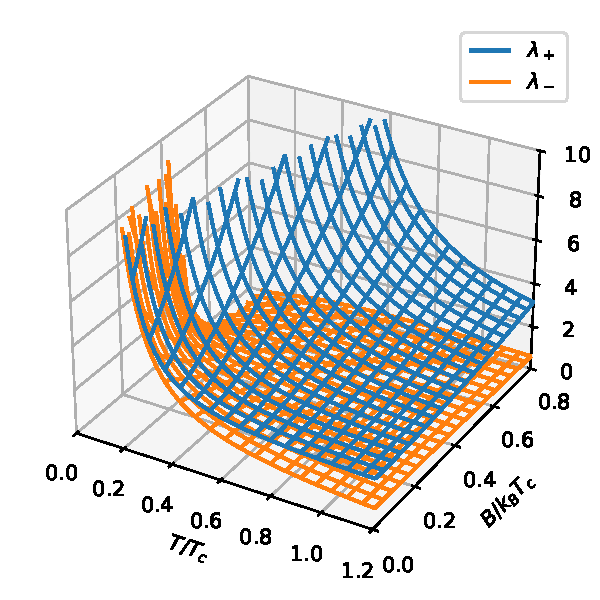
\includegraphics[scale=0.8]{figures/plot of lambda_+ and lambda_-.pdf}
			\caption{plot of $\lambda_\pm(T, B)$.}
		\end{figure}
		
		\item 注意到
		\begin{equation}
			\lambda_-(T \rightarrow 0, B) = e^{\beta (J - B)} = \begin{dcases}
				\infty & B < J \\
				1 & B = J \\
				0 & B > J
			\end{dcases}.
		\end{equation}
	\end{itemize}
	
	\item 得到
	\begin{equation}
		\braket{m} = \frac{1}{N \beta} \frac{\partial}{\partial B} \ln Z_\text{C} = \frac{e^{\beta J} \sinh \beta B}{\sqrt{e^{2 \beta J} \cosh^2 \beta B - 2 \sinh 2 \beta J}},
	\end{equation}
	并注意到
	\begin{equation}
		\braket{m}(T, B = 0) = 0.
	\end{equation}
	
	\item $\braket{m}(T, B)$ 的函数图像如下:
	
	\begin{figure}[H]
		\centering
		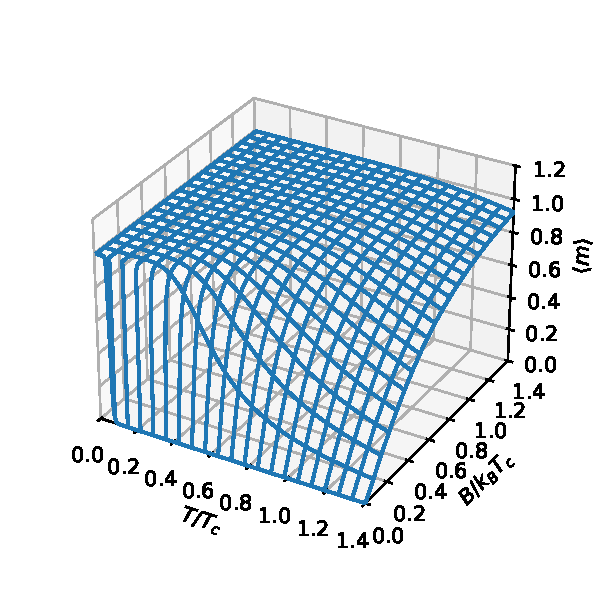
\includegraphics[scale=0.8]{figures/plot of the magnetization.pdf}
		\caption{plot of the magnetization.}
	\end{figure}
	
	\item 可见, Ising chain 中不存在 phase transition, 与 mean field theory 预测的结果完全不同.
\end{itemize}

\subsection{2-dim. Ising model: low temperatures and Peierls droplets}
\begin{itemize}
	\item 考虑 $B = 0, T \rightarrow 0$ 下的 2-dim. square lattice.
	
	\item 2-dim. Ising model 的最低 3 个能级如下图所示:
	
	\begin{figure}[H]
		\centering
		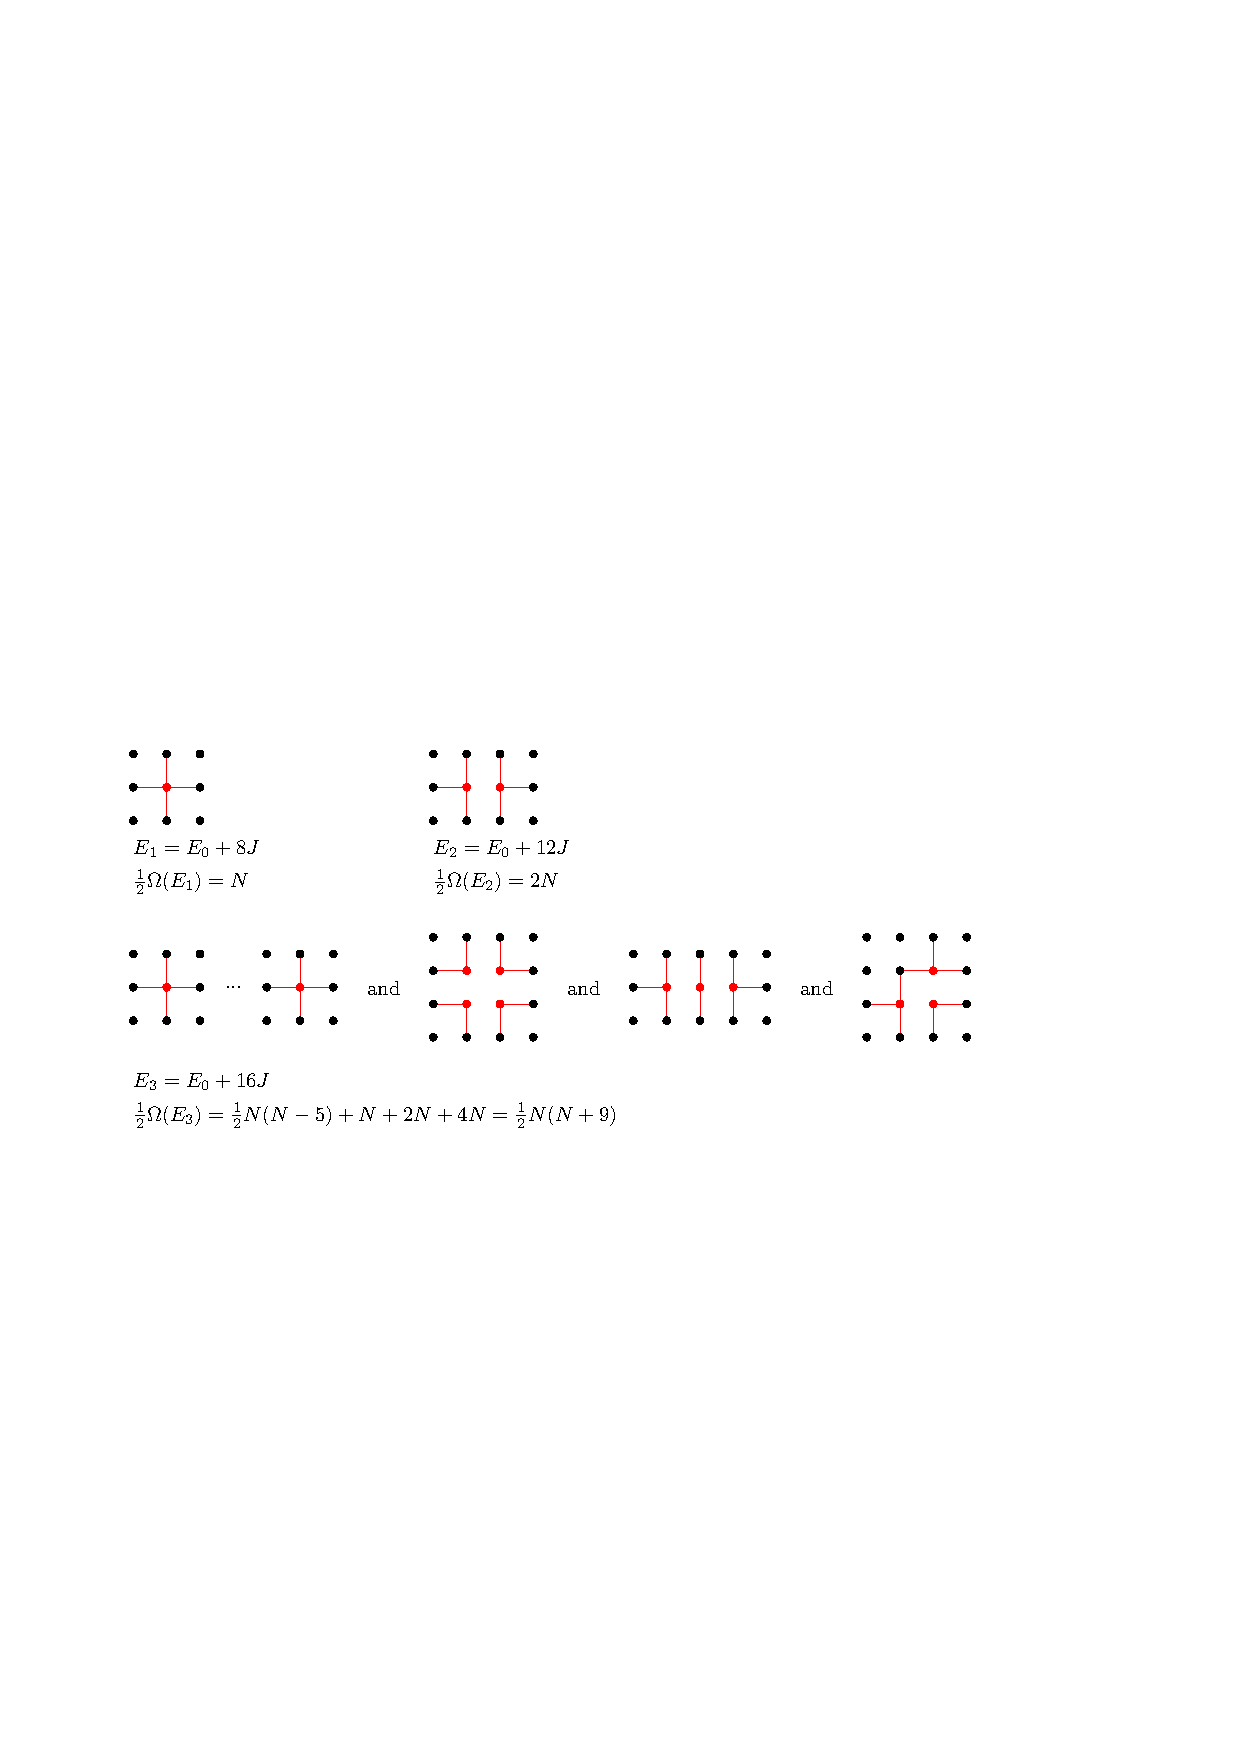
\includegraphics[scale=1]{figures/lowest 3 energy levels of the 2-dim. Ising model.pdf}
		\caption{lowest 3 energy levels of the 2-dim. Ising model.}
	\end{figure}
	
	\item 因此, 低温下近似有
	\begin{equation}
		Z_\text{C} = 2 e^{- \beta E_0} \Big( 1 + N e^{- 8 \beta J} + 2 N e^{- 12 \beta J} + \frac{1}{2} N (N + 9) e^{- 16 \beta J} + \cdots \Big),
	\end{equation}
	其中 $E_0 = - 2 N J$, 并注意到 $\Omega(E_0) = 2$.
	
	\item 系统的 Helmholtz free energy 为 (注意 $\ln(1 + x) = x - \frac{x^2}{2} + \cdots$)
	\begin{align}
		- \beta F &= \ln Z_\text{C} \notag \\
		&= \ln 2 + 2 N \beta J + \Big( N e^{- 8 \beta J} + 2 N e^{- 12 \beta J} + \frac{1}{2} N (N + 9) e^{- 16 \beta J} + \cdots \Big) - \frac{1}{2} N^2 e^{- 16 \beta J} + \cdots \notag \\
		&= \ln 2 + 2 N \beta J + \Big( N e^{- 8 \beta J} + 2 N e^{- 12 \beta J} + \frac{9}{2} N e^{- 16 \beta J} + \cdots \Big),
	\end{align}
	可见 $F \propto N$.
	
	\item general lesson: partition function can be written as the exponential of the sum of \textbf{connected diagrams}.
\end{itemize}

\subsection{Peierls droplets}
\begin{itemize}
	\item 
\end{itemize}
